%
% einleitung.tex -- Beispiel-File für die Einleitung
%
% (c) 2020 Prof Dr Andreas Müller, Hochschule Rapperswil
%
\section{Problem\label{parzyl:section:teil0}}
\rhead{Teil 0}

\subsection{Laplace Gleichung}
Die partielle Differentialgleichung
\begin{equation}
    \Delta f = 0
\end{equation}
ist als Laplace Gleichung bekannt.
Sie ist eine spezielle Form der poisson Gleichung
\begin{equation}
    \Delta f = g
\end{equation}
mit g als beliebige Funktion.
In der Physik hat die Laplace Gleichung in verschieden Gebieten
verwendet, zum Beispiel im Elektromagnetismus.
Das Gaussche Gesetz in den Maxwellgleichungen 
\begin{equation}
     \nabla \cdot E = \frac{\varrho}{\epsilon_0}
\label{parzyl:eq:max1}
\end{equation}
besagt das die Divergenz eines Elektrischen Feldes an einem 
Punkt gleich der Ladung an diesem Punkt ist.
Das elektrische Feld ist hierbei der Gradient des elektrischen
Potentials
\begin{equation}
    \nabla \phi = E.
\end{equation}
Eingesetzt in \eqref{parzyl:eq:max1} resultiert
\begin{equation}
    \nabla \cdot \nabla \phi = \Delta \phi = \frac{\varrho}{\epsilon_0},
\end{equation}
was eine Possion gleichung ist.
An Ladungsfreien Stellen, ist der rechte Teil der Gleichung $0$. 
\subsection{Parabolische Zylinderkoordinaten
\label{parzyl:subsection:finibus}}
Im parabloischen Zylinderkoordinatensystem bilden parabolische Zylinder die Koordinatenflächen.
Die Koordinate $(\sigma, \tau, z)$ sind in kartesischen Koordinaten ausgedrückt mit
\begin{align}
    x & = \sigma \tau \\
    y & = \frac{1}{2}\left(\tau^2 - \sigma^2\right) \\
    z & = z.
\end{align}
Wird $\tau$ oder $\sigma$ konstant gesetzt reultieren die Parabeln
\begin{equation}
    y = \frac{1}{2} \left( \frac{x^2}{\sigma^2} - \sigma^2 \right)
\end{equation}
und 
\begin{equation}
    y = \frac{1}{2} \left( -\frac{x^2}{\tau^2} + \tau^2 \right).
\end{equation}

\begin{figure}
    \centering
    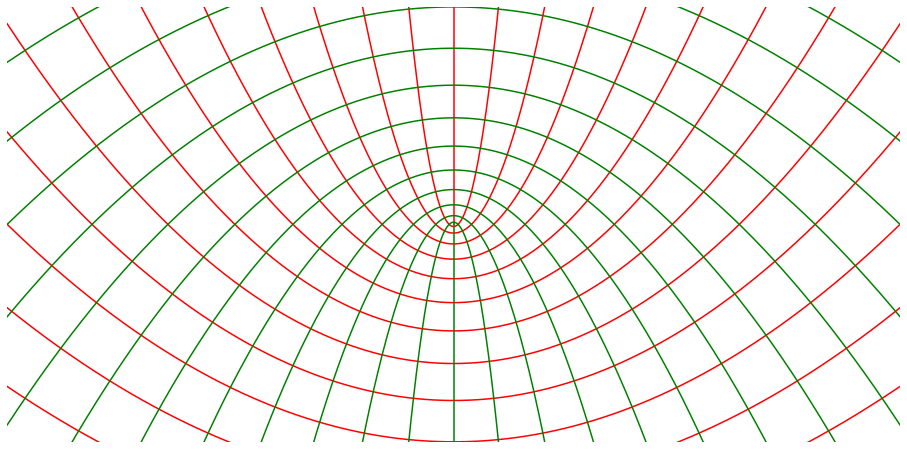
\includegraphics[scale=0.4]{papers/parzyl/img/koordinaten.png}
    \caption{Das parabolische Koordinatensystem. Die roten Parabeln haben ein 
    konstantes $\sigma$ und die grünen ein konstantes $\tau$.}
    \label{fig:cordinates}
\end{figure}

Abbildung \ref{fig:cordinates} zeigt das Parabolische Koordinatensystem.
Das parabolische Zylinderkoordinatensystem entsteht wenn die Parabeln aus der
Ebene gezogen werden. 

\subsection{Differnetialgleichung}
Lorem ipsum dolor sit amet, consetetur sadipscing elitr, sed diam
nonumy eirmod tempor invidunt ut labore et dolore magna aliquyam
erat, sed diam voluptua \cite{parzyl:bibtex}.
At vero eos et accusam et justo duo dolores et ea rebum.
Stet clita kasd gubergren, no sea takimata sanctus est Lorem ipsum
dolor sit amet.

Lorem ipsum dolor sit amet, consetetur sadipscing elitr, sed diam
nonumy eirmod tempor invidunt ut labore et dolore magna aliquyam
erat, sed diam voluptua.
At vero eos et accusam et justo duo dolores et ea rebum.  Stet clita
kasd gubergren, no sea takimata sanctus est Lorem ipsum dolor sit
amet.


